\documentclass[12pt]{article}
\usepackage[T1]{fontenc}
\usepackage[utf8]{inputenc}
\usepackage[spanish]{babel}
\decimalpoint
\usepackage{amsmath}
\usepackage{amsfonts}
\usepackage{amssymb}
\usepackage{supertabular}
\usepackage{float}
\usepackage{graphicx}
\usepackage{subcaption}
\usepackage[margin=2cm]{geometry}
\usepackage{multirow}
\usepackage[hidelinks]{hyperref}
%\usepackage{breqn}
\graphicspath{ {figuras/} }

\author{Guillermo Xchell Calva García}
\title{\textbf{Inestabilidades electrostáticas debidas a haces de partículas.}}
\date{}
\begin{document}
\maketitle
Para tratar el tema de inestabilidades se mostrará primero que frecuencias complejas pueden aparecer en el plasma si se tiene un arreglo de haces de partículas adecuado \cite{bellan2008fundamentals}.\\
%The first part of this chapter develops some
%preparatory ideas by showing that complex frequencies, i.e., wave instabilities,
%can develop if there are suitably arranged particle beams in a plasma.
El tratatamiento inicial se hará desde la perspectiva de fluidos. Se parte entonces de las siguientes ecuaciones:
\begin{equation}
\label{cont_nl}
\frac{\partial n_{\sigma}}{\partial t} + \overrightarrow{\nabla} \cdot n_{\sigma}\overrightarrow{\textbf{u}}_{\sigma}=0
\end{equation}
\begin{equation}
\label{eq_movimiento_nl}
n_{\sigma}m_{\sigma}\frac{d\overrightarrow{\textbf{u}}_{\sigma}}{dt}= n_{\sigma}q_{\sigma}(\overrightarrow{\textbf{E}} + \overrightarrow{\textbf{u}}_{\sigma} \times \overrightarrow{\textbf{B}}) - \nabla P_{\sigma} - \textbf{R}_{\sigma \alpha}
\end{equation}
\begin{equation}
\label{poisson_nl}
\nabla ^2 \Phi = -\frac{1}{\epsilon_0}\sum _{\sigma}q_{\sigma} n_{\sigma}
\end{equation}
Las cuales son respectivamente la ecuación de continuidad, movimiento y Poisson para cada especie. Al tratarse del caso electróstatico la ecuación \ref{eq_movimiento_nl} se puede reducir a la siguiente forma:
\begin{equation}
\label{eq_mov_simpl_nl}
n_{\sigma}m_{\sigma}\frac{d\overrightarrow{\textbf{u}}_{\sigma}}{dt}= n_{\sigma}q_{\sigma} \overrightarrow{\textbf{E}}
\end{equation}
Con $\overrightarrow{\textbf{E}} = - {\overrightarrow\nabla} \Phi$. Y donde se han despreciado los términos de aceleración debido al campo magnético (puesto que ese término es cero para modos longitudinales), la presión y a la fuerza de fricción debida a colisiones. Además, se tiene $d/dt \equiv \partial / \partial t + \overrightarrow{\textbf{u}}_{\sigma} \cdot \overrightarrow{\nabla}$, la cual se le conoce como la derivada convectiva.\\
%Los términos $\nabla P_{\sigma}$ y $\textbf{R}_{\sigma \alpha}$ se refieren a la presión y a la fuerza de fricción resultante de las colisiones entre las especies $\sigma$ y $\alpha$ respectivamente.\\
El siguiente paso entonces es introducir un método que permita ver el comportamiento de las ondas longitudinales en el  plasma debido a cada una de las especies. Dicho método se le conoce como análisis lineal y el procedimiento es el siguiente:
\begin{itemize}
\item Se reduce el sistema a un simple conjunto de ecuaciones que describan su comportamiento.
\item Se determina una solución de equilibrio para las ecuaciones y a las cantidades de equilibrio se les designa con el subíndice 0, indicando que son cantidades de orden cero.
\item Si $\lbrace f(\textbf{x},t), g(\textbf{x},t),h(\textbf{x},t),...\rbrace$ es el conjunto de las variables dependientes y se le agrega una perturbación a una de las variables, entonces al resolver el sistema de ecuaciones se obtendrá la respuesta de las otras variables a la perturbación. Supongasé que se le agrega una perturbación $\epsilon f_1$ a la variable $f$, con $\epsilon \ll 1$ entonces se tiene:
\begin{equation*}
f = f_0 + \epsilon f_1
\end{equation*}
El sistema entonces da la dependencia funcional de las otras variables, por ejemplo $g = g(f) = g(f_0 + \epsilon f_1)$. Dado que ésta dependencia por lo general es no lineal la expansión de Taylor da $g = g_0 + \epsilon g_1 + \epsilon^2 g_2 + \epsilon^3 g_3 +...$ Si se considera a las epsilons como coeficientes implícitos las variables se pueden escribir entonces como:
$$
\begin{array}{lllllllll}
f &= &f_0 &+ &f_1 \\
g &= &g_0 &+ &g_1 &+ &g_2 &+ &...\\
h &= &h_0 &+ &h_1 &+ &h_2 &+ &...
\end{array}
$$
\item Se reescriben entonces las ecuaciones del sistema con las variables expandidas a primer orden y se discriminan los términos de segundo orden resultantes, así como también haciendo uso de las soluciones de equilibrio para simplificar las expresiones.
\end{itemize}
Para el caso de la ecuación de continuidad se tiene entonces:
\begin{equation}
\frac{\partial (n_{\sigma 0} + n_{\sigma 1})}{\partial t} + \overrightarrow{\nabla} \cdot [(n_{\sigma 0}+n_{\sigma 1})(\overrightarrow{\textbf{u}}_{\sigma 0} + \overrightarrow{\textbf{u}}_{\sigma 1})]=0
\end{equation}
Donde la solución de equiibrio es:
\begin{equation}
\frac{\partial n_{\sigma 0}}{\partial t} + \overrightarrow{\nabla} \cdot n_{\sigma 0}\overrightarrow{\textbf{u}}_{\sigma 0}=0
\end{equation}
Lo que da:
\begin{equation}
\frac{\partial n_{\sigma 1}}{\partial t}+ \overrightarrow{\nabla} \cdot (n_{\sigma 1} \overrightarrow{\textbf{u}}_{\sigma 0} + n_{\sigma 0} \overrightarrow{\textbf{u}}_{\sigma 1} + n_{\sigma 1} \overrightarrow{\textbf{u}}_{\sigma 1}) =0
\end{equation}
El término $n_1 \overrightarrow{\textbf{u}}_1$ es de segundo orden y por lo tanto se descarta. Con lo que la ecuación de continuidad linealizada es:
\begin{equation}
\label{cont_lin}
\frac{\partial n_{\sigma 1}}{\partial t}+ \overrightarrow{\nabla} \cdot (n_{\sigma 1} \overrightarrow{\textbf{u}}_{\sigma 0} + n_{\sigma 0} \overrightarrow{\textbf{u}}_{\sigma 1}) =0
\end{equation}
De manera similar, las ecuaciones de movimiento y de Poisson son linealizadas para dar:
\begin{equation}
\label{eq_mov_lin}
\frac{\partial \overrightarrow{\textbf{u}}_{\sigma 1}}{\partial t} + \overrightarrow{\textbf{u}}_{\sigma 0} \cdot \overrightarrow{\nabla}\overrightarrow{\textbf{u}}_{\sigma 1} = - \frac{q_{\sigma}}{m_{\sigma}} \overrightarrow{\nabla}\Phi _1
\end{equation}
\begin{equation}
\label{poisson_lin}
\nabla ^2 \Phi _1 = -\frac{1}{\epsilon_0}\sum _{\sigma}q_{\sigma} n_{\sigma 1}
\end{equation}
Recordando que lo que se quiere estudiar está en el marco de ondas longitudinales en el plasma se considera que la perturbación lineal es un modo de Fourier. Por lo cual las variables cambian de la misma manera en la que lo haría exp ($i \overrightarrow{\textbf{k}} \cdot \overrightarrow{\textbf{x}} - i \omega t $), es decir $\overrightarrow{\nabla} \rightarrow i\overrightarrow{\textbf{k}}$ y $\partial / \partial t \rightarrow -i \omega$ por lo que las ecuaciones \ref{cont_lin}, \ref{eq_mov_lin} y \ref{poisson_lin} se pueden reescribir como:
\begin{equation}
\label{cont_fourier}
 -i \omega n_{\sigma 1}+ i\overrightarrow{\textbf{k}} \cdot (n_{\sigma 1} \overrightarrow{\textbf{u}}_{\sigma 0} + n_{\sigma 0} \overrightarrow{\textbf{u}}_{\sigma 1}) =0
\end{equation}
\begin{equation}
\label{eq_mov_fourier}
-i \omega \overrightarrow{\textbf{u}}_{\sigma 1} + \overrightarrow{\textbf{u}}_{\sigma 0} \cdot i \overrightarrow{\textbf{k}}\overrightarrow{\textbf{u}}_{\sigma 1} = - \frac{i q_{\sigma}}{m_{\sigma}} \overrightarrow{\textbf{k}}\Phi _1
\end{equation}
\begin{equation}
\label{poisson_fourier}
-k^2 \Phi _1 = -\frac{1}{\epsilon_0}\sum _{\sigma}q_{\sigma} n_{\sigma 1}
\end{equation}
Si se fatoriza el término de primer orden de la velocidad en la ecuación de movimiento se obtiene:
\begin{equation}
\label{U1}
\overrightarrow{\textbf{u}}_{\sigma 1} = \frac{- i q_{\sigma} k \Phi _1}{m_{\sigma}(-i \omega + \overrightarrow{\textbf{u}}_{\sigma 0} \cdot i \overrightarrow{\textbf{k}})}
\end{equation}
Al sustituir \ref{U1} en \ref{cont_fourier} se obtiene:
\begin{equation}
n_{\sigma 1} = n_{\sigma 0}\frac{k^2 q_{\sigma} \Phi _1  }{m_{\sigma}(\omega - \overrightarrow{\textbf{u}}_{\sigma 0} \cdot \overrightarrow{\textbf{k}})^2 }
\end{equation}
La cual a su vez se sustituye en \ref{poisson_fourier} y recordando que $\omega_{p \sigma}^2 = q_{\sigma}^2 n_{\sigma 0} / m_{\sigma} \epsilon_0$ se llega a:
\begin{equation}
\label{eq_dispersion}
1 = \sum_{\sigma} \frac{\omega_{p \sigma}^2}{(\omega - \overrightarrow{\textbf{u}}_{\sigma 0} \cdot \overrightarrow{\textbf{k}})^2}
\end{equation}
A la expresión resultante se le conoce como la relación de dispersión. Se tienen entonces las herramientas necesarias para este primer estudio de inestabilidades en un plasma para distintas configuraciones de haces.\\
Debido a que la ecuación \ref{eq_dispersion} parte de la ecuación de Poisson se puede inferir que la relación de dispersión es equivalente a una expresión para la permitividad eléctrica. Para ver esto se recuerda que
$\nabla ^2 \Phi _1 = - \nabla \cdot \overrightarrow{\textbf{E}}$ o en este caso $-k^2 \Phi _1 = -i \overrightarrow{\textbf{k}} \cdot \overrightarrow{\textbf{E}}$ por lo que se puede escribir:
\begin{equation}
-i \overrightarrow{\textbf{k}} \cdot \overrightarrow{\textbf{E}} = - \sum \frac{\omega_{p \sigma}^2 k^2 \Phi _1}{(\omega - \overrightarrow{\textbf{u}}_{\sigma 0} \cdot \overrightarrow{\textbf{k}})^2} = - \sum \frac{\omega_{p \sigma}^2 (i \overrightarrow{\textbf{k}} \cdot \overrightarrow{\textbf{E}})}{(\omega - \overrightarrow{\textbf{u}}_{\sigma 0} \cdot \overrightarrow{\textbf{k}})^2}
\end{equation}
Factorizando términos se llega a:
\begin{equation}
\label{eq:gauss_dilectric_omega}
i \overrightarrow{\textbf{k}} \cdot \overrightarrow{\textbf{E}} \left( 1 - \sum \frac{\omega_{p \sigma}^2 }{(\omega - \overrightarrow{\textbf{u}}_{\sigma 0} \cdot \overrightarrow{\textbf{k}})^2} \right) = 0
\end{equation}
La ecuación \ref{eq:gauss_dilectric_omega} se puede ver como un caso especial de la ley de Gauss para dieléctricos en donde $\nabla \cdot \overrightarrow{\textbf{D}}=0$, donde además si se tiene $\overrightarrow{\textbf{D}}= \epsilon \overrightarrow{\textbf{E}}$ con $\epsilon = 1+ \chi$, siendo $\chi$ la susceptibilidad eléctrica, el término del lado derecho de la ecuación \ref{eq_dispersion} se puede ver como la suma de las susceptibilidades de las diferentes especies.
\begin{equation}
\label{eq:suma_susceptibilidades}
\sum \chi _\sigma = - \sum_{\sigma} \frac{\omega_{p \sigma}^2}{(\omega - \overrightarrow{\textbf{u}}_{\sigma 0} \cdot \overrightarrow{\textbf{k}})^2}
\end{equation}
Las expresiones aquí obtenidas son generalizadas, a continuación se presentará el estudio de algunos casos particulares.
\subsection*{Caso con $\omega_{p\sigma}^2$ iguales y velocidades de flujo de signo contrario.}
El caso más simple es el de dos especies con la misma frecuencia de plasma al cuadrado y velocidades de flujo iguales en magnitud pero de signo contrario. Este caso podría referirse a dos haces de electrones, dos haces de iones o un haz de electrones y otro de positrones con velocidades de signo contrario. En cualquiera de estos casos la relación de dispersión queda como:
\begin{equation}
\label{dispersion_ep}
1= \frac{\omega_{p\sigma}^2}{(\omega - \overrightarrow{\textbf{u}}_{\sigma 0} \cdot \overrightarrow{\textbf{k}})^2} + \frac{\omega_{p\sigma}^2}{(\omega + \overrightarrow{\textbf{u}}_{\sigma 0} \cdot \overrightarrow{\textbf{k}})^2}
\end{equation}
Ahora bien, si se definen $z= \omega / \omega_{p\sigma}$ y $\lambda = \overrightarrow{\textbf{k}} \cdot \overrightarrow{\textbf{u}}_{\sigma 0}/ \omega_{p\sigma}$ y se substituyen en la ecuación anterior se llega a la expresión:
\begin{equation}
\label{dispersion_ep_adimensional}
1 = \frac{1}{(z - \lambda)^2} + \frac{1}{(z + \lambda)^2}
\end{equation}
El siguiente paso es desarrollar la ecuación pero nótese que en el lado derecho de la ecuación hay singularidades en $z= \pm \lambda$ es decir dependiendo del valor que se tenga de $\lambda$ se determinará el mínimo de $z(\lambda)$ en la región $(- \lambda, \lambda)$. Con esto en mente se prosigue a desarrollar la ecuación \ref{dispersion_ep_adimensional}.
\begin{equation}
z^4 -2z^2(\lambda^2 + 1) +\lambda ^4 -2 \lambda ^2 =0
\end{equation}
Donde al resolver para $z^2$ se llega a:
\begin{equation}
\label{bicaudratica_ep}
z^2= (\lambda^2 +1) \pm (4 \lambda ^2 + 1)^{1/2}
\end{equation}
La elección del signo determinará dos raíces de $z$, si $z^2 >0$ las raíces son reales, de la misma magnitud pero signo opuesto. En cambio si $z^2 <0$ las dos raíces son imaginarias, conjugadas. Recordando la definición de $z$ y la forma en la que varía la perturbación se llega entonces  a la conclusión de que la raíz imaginaria positiva corresponde a una perturbación que crece exponencialmente con el tiempo, es decir a una inestabilidad. Con este fin se escoje el signo negativo en la ecuación \ref{bicaudratica_ep} entonces se tiene que la condición para la inestabilidad es:
\begin{equation}
(4 \lambda ^2 + 1)^{1/2} > (\lambda^2 +1 )
\end{equation}
O de manera más simple:
\begin{equation}
0 < \lambda < \sqrt{2}
\end{equation}
Una vez conseguido esto, lo siguiente sería encontrar la máxima tasa de crecimiento de la inestabilidad. Para ello se maximizará  la ecuación \ref{bicaudratica_ep} con respecto a $\lambda$ haciendo entonces el término $dz/d \lambda = 0$ queda
\begin{equation}
2 \lambda - \frac{4 \lambda}{(4 \lambda ^2 + 1)^{1/2}}=0
\end{equation}
Que simplificando es:
\begin{equation}
(4 \lambda ^2 + 1)^{1/2} = 2
\end{equation}
Del cual se obtiene $\lambda = \sqrt{3} / 2$. Sustituyendo en la ecuación \ref{bicaudratica_ep} se obtiene $z = i / 2$.\\
Regresando a las variables físicas, se tiene que el umbral de inestabilidad es:
\begin{equation}
ku_0 < \sqrt{2}\omega_{p \sigma}
\end{equation}
Mientras que la máxima tasa de crecimiento resulta ocurrir cuando:
\begin{equation}
ku_0 = \frac{\sqrt{3}}{2}\omega_{p \sigma}
\end{equation}
Por lo que se tiene:
\begin{equation}
\omega  = i \frac{ \omega_{p \sigma}}{2}
\end{equation}
Finalmente, para poder ver el comportamiento de la tasa de crecimiento en función de $\lambda$ se calcula entonces la raíz de la ecuación \ref{bicaudratica_ep}, obteniendo la expresión siguiente:
\begin{equation}
\label{eq:z_misma_omega}
z = \pm \sqrt{(\lambda^2 +1) - (4 \lambda ^2 + 1)^{1/2}}
\end{equation}
En donde como ya se había mencionado, lo que se busca es la raíz con la componente imaginaria positiva, por lo que se escoge el signo positivo en la ecuación \ref{eq:z_misma_omega}. La figura \ref{fig:misma_omega_tasa_de_crecimiento} muestra entonces la tasa de crecimiento de inestabilidad Im$z$ como función de $\lambda$.
\begin{figure}
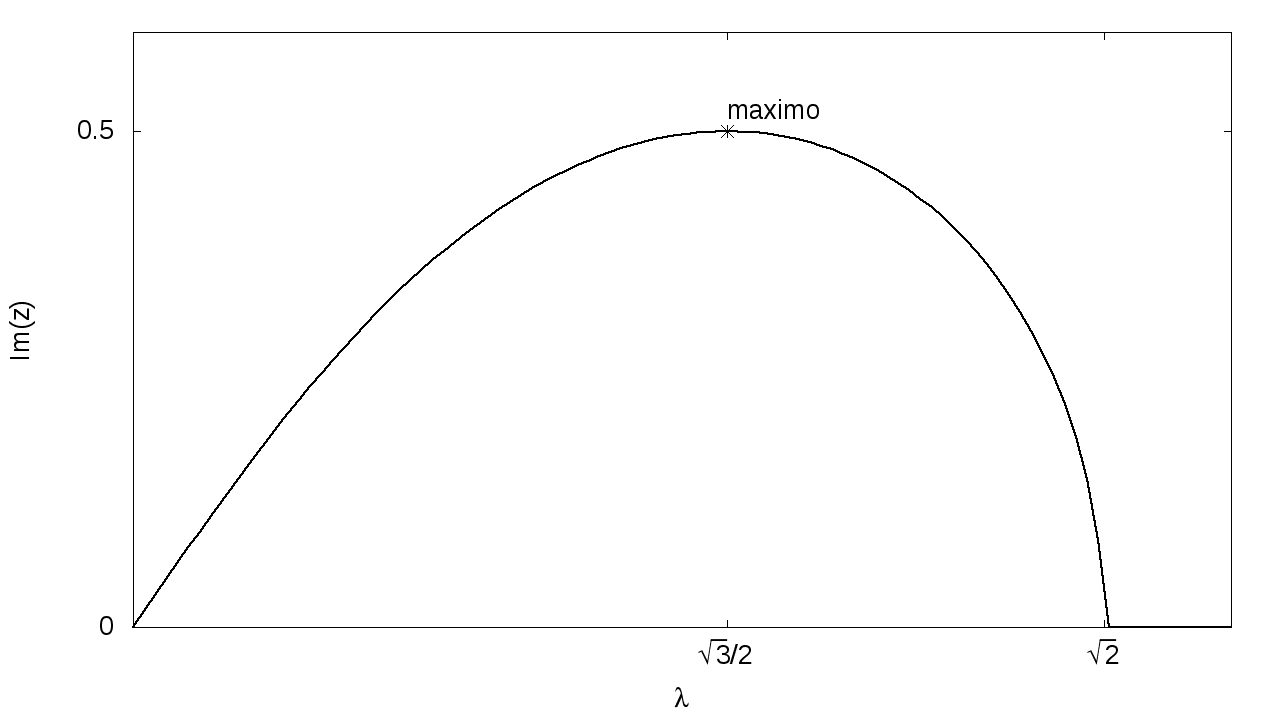
\includegraphics[height=0.3\paperheight]{grafica_misma_omega_contrarias.png}
\caption{tasa de crecimiento para dos especies con misma $\omega_{p\sigma}^2$ pero con velocidades de signo contrario.}
\label{fig:misma_omega_tasa_de_crecimiento}
\end{figure}
\subsection*{Caso misma $\omega_{p\sigma}$ con una especie incidente y la otra estacionaria.}
La relación de dispersión para este caso es muy similar a la ecuación \ref{dispersion_ep_adimensional}, el único cambio se da en recordar que una de las especies tiene velocidad cero, por lo tanto se tiene:
\begin{equation}
\label{eq:misma_omega_reposo}
1 = \frac{1}{z^2} + \frac{1}{(z-\lambda)^2}
\end{equation}
Al igual que el caso de dos especies con misma $\omega_{p\sigma}^2$ pero con velocidades de signo contrario, la raíz que nos es de interes es la raíz cuya parte imaginaria sea positiva, es decir en donde la perturbación crece exponencialmente con el tiempo. Para resolver la raíz se emplea el cambio de variable $z=x+\frac{\lambda}{2}$ lo que resulta en la siguiente expresión:
\begin{equation}
\label{eq:reducida_misma_reposo}
x^4 - \frac{1}{2}(4 + \lambda^2)x^2 + \frac{1}{16}\lambda^2 (\lambda^2 -8)=0
\end{equation}
La cuál es una ecuación bicuadrática de $x$ que permite entonces escribir:
\begin{equation}
\label{eq:bicuad_misma_reposo}
x^2 = \frac{1}{4}(4 + \lambda^2 \pm 4\sqrt{ \lambda^2 +1})
\end{equation}
De la cual se calcula la raíz para $x$ y se realiza el cambio de variable correspondiente para recuperar una solución en $z$.
\begin{equation}
\label{eq:solucion_misma_reposo}
z = \frac{1}{2}\left(\lambda + \sqrt{4 + \lambda ^2 - 4 \sqrt{1 + \lambda ^2}} \right)
\end{equation}
Los signos de la raíz se escogen para que la parte imaginaria de $z$ sea positiva. Para más detalle sobre la obtención de la raíz véase el apéndice \ref{Ap:raices}.
El siguiente paso es buscar el umbral en donde sucede la inestabilidad y para ello se estudia el lado derecho de la ecuación \ref{eq:misma_omega_reposo} y se observa que tiene dos singularidades $z=0,\lambda$. Aquí, el valor de $\lambda$ determinará el mínimo del lado derecho de \ref{eq:misma_omega_reposo} en el intervalo $(0,\lambda)$, al cual llamaremos $f(z,\lambda)$ por simplicidad. La figura \ref{fig:fz_reposo} ilustra el caso para una cierta $\lambda$, en donde se puede apreciar como el valor de $\lambda$ puede afectar el mínimo en el intervalo $(0,\lambda)$. El mínimo que nos interesa es el de valor $1$ pues ese índica cuando las raíces de ecuación \ref{eq:misma_omega_reposo} empizan a ser imaginarias. Estrictamente hablando, cuando el mínimo es uno quiere decir que dos de sus raíces reales se vuelven una y es cuando el mínimo es mayor que uno que aparecen raíces imaginarias.
\begin{figure}
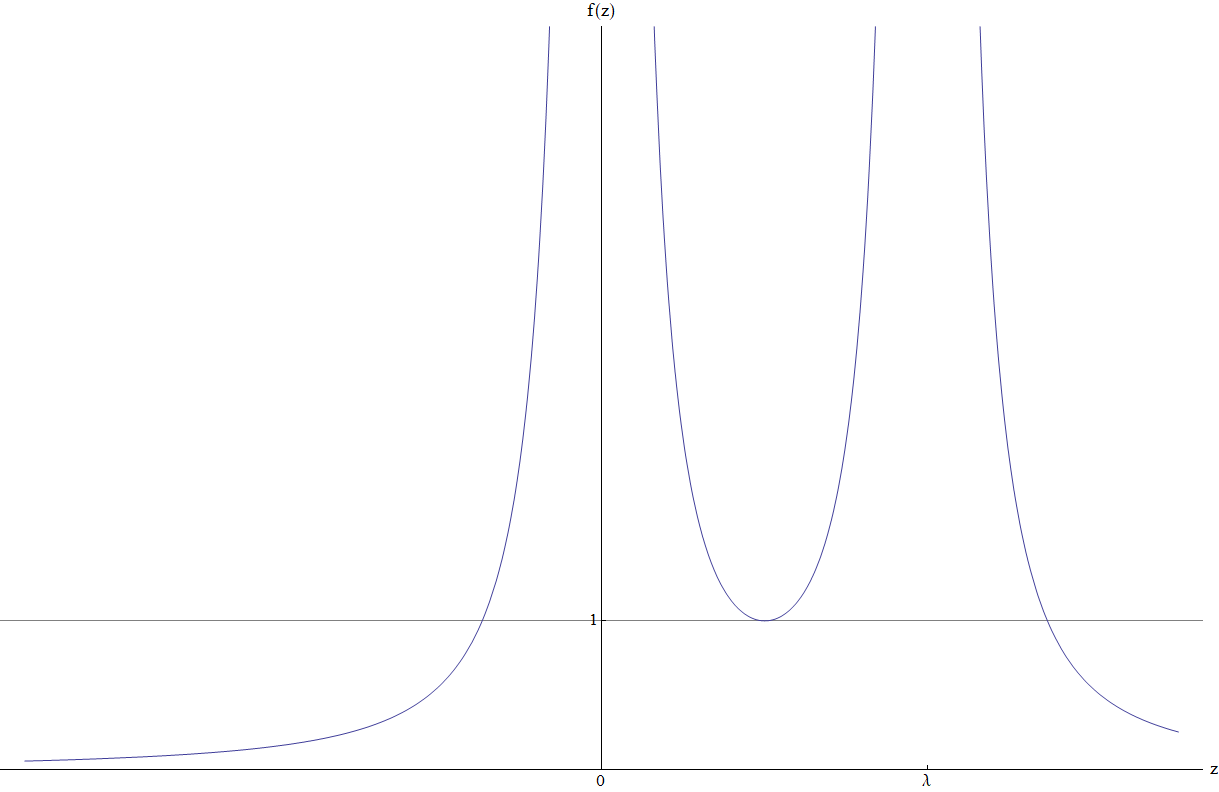
\includegraphics[height=0.3\paperheight]{f_z_reposo.png}
\caption{gráfica del lado derecho de la ecuación \ref{eq:misma_omega_reposo} para un cierto valor de $\lambda$}
\label{fig:fz_reposo}
\end{figure}
Para encontrar ese umbral se busca entonces para que $\lambda$s el mínimo de $f(z,\lambda)$ es igual a uno. Se empieza entonces por minimizar.
\begin{equation}
\frac{1}{z^3} + \frac{1}{(z-\lambda)^3}=0
\end{equation}
El cual da $z=\lambda / 2$. Que al sustituir en \ref{eq:misma_omega_reposo} y resolver para $\lambda$ da $\lambda = \sqrt{8}$. Por lo que se tiene que el intervalo de inestabilidad es:
\begin{equation}
0 < \lambda < \sqrt{8}
\end{equation}
Para encontrar la máxima tasa de crecimiento se hace uso de que la ecuación \ref{eq:solucion_misma_reposo} representa un número complejo. Basta entonces buscar el máximo de la norma de dicho número. Se tiene entonces:
\begin{equation}
|z|^2 = \frac{1}{4}[\lambda^2 -4 - \lambda^2 + 4(1 + \lambda^2)^{1/2}]
\end{equation}
Donde al observar la ecuación \ref{eq:solucion_misma_reposo} vemos que los términos que le corresponden a la parte imaginaria son $-4 - \lambda^2 + 4(1 + \lambda^2)^{1/2}$. Es decir si $z=x +iy$:
\begin{equation}
y^2= -4 - \lambda^2 + 4(1 + \lambda^2)^{1/2}
\end{equation}
Que al maximizar con respécto de $\lambda$ da:
\begin{equation}
2\lambda -\lambda(1 + \lambda^2)^{1/2} =0
\end{equation}
Y al resolver para $\lambda$ se obtiene
\begin{equation}
\lambda = \sqrt{3}
\end{equation}
Estos valores se pueden apreciar en la figura \ref{fig:misma_omega_tasa_de_crecimiento} que grafica la parte imaginaria de $z$, es decir la correspondiente al crecimiento de la inestabilidad, contra $\lambda$. 
\begin{figure}[!h]
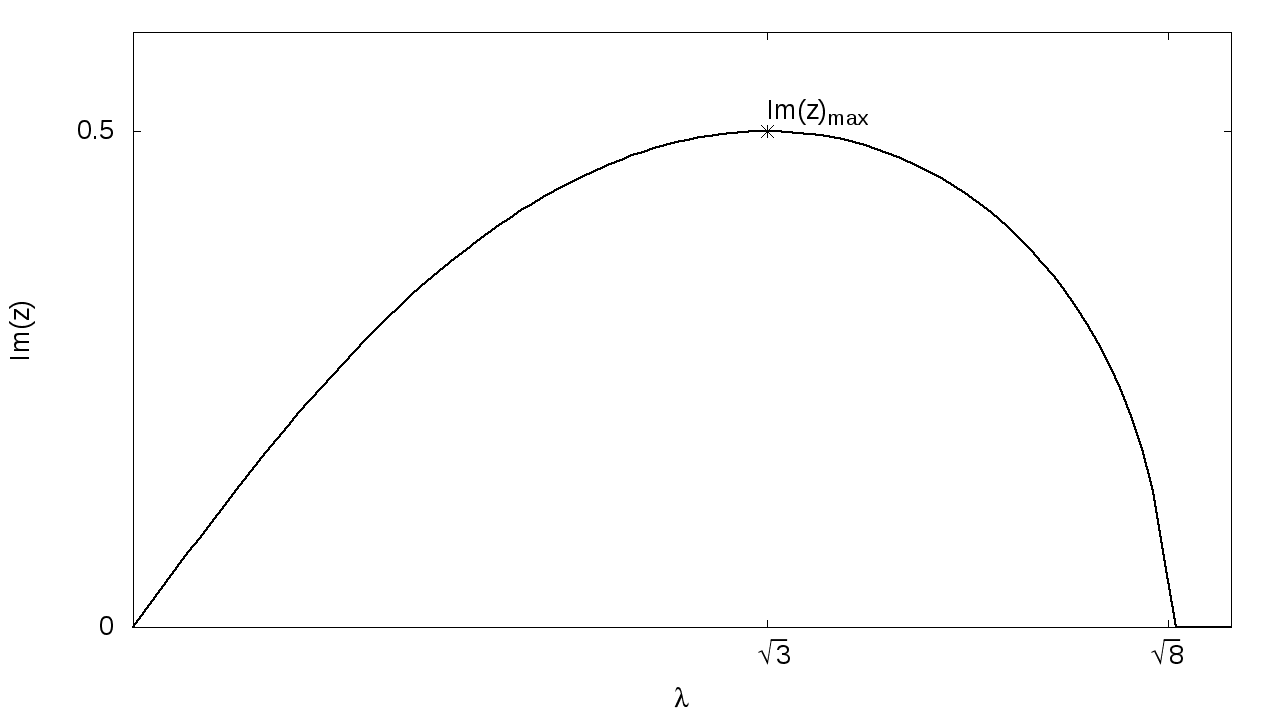
\includegraphics[height=0.3\paperheight]{grafica_misma_omega_reposo.png}
\caption{tasa de crecimiento para dos especies con misma $\omega_{p\sigma}^2$ pero una de ellas estacionaria.}
\label{fig:misma_omega_reposo}
\end{figure}
Ahora bien regresando a variables físicas se tiene que el umbral de insetabilidad ocurre cuando
\begin{equation}
ku_0 < \sqrt{8} \omega_{p\sigma}
\end{equation}
Y la máxima tasa de crecimiento sucede cuando:
\begin{equation}
ku_0= \sqrt{3} \omega_{p\sigma}
\end{equation}
Y en cuyo caso se tiene
\begin{equation}
\omega = \frac{1}{2} (\sqrt{3} + i)\omega_{p\sigma}
\end{equation}
\subsection*{Generalizando el caso para dos especies con la misma $\omega_{p\sigma}$}
Como se vió en el caso para mismas especies con velocidades opuestas, la relación de dispersión se reduce a una ecuación bicuadrática y de esa manera se encuentran las raíces de la ecuación cuártica. Ésta reducción es posible debido a la simetría del problema. Sin embargo, se tiene que al encontrar las raíces de la ecuación cuártica para el caso de una especie en reposo y otra especie incidente con cierta velocidad arbitraria, también se llega a una ecuación bicuadrática a pesar de no tener la misma simetría que el caso con dos velocidades opuestas. Dicha ecuación bicuadrática aparece como resultado de un cambio de variable $z=x+\lambda /2$, para más detalle véase el apéndice \ref{Ap:raices}. Esto podría sugerir que para dos especies con la misma $\omega_{p\sigma}$ su relación de dispersión siempre se puede reducir a una ecuación bicuadrática con el cambio de variable apropiado. Independientemente de la velocidad que lleve cada especie.\\
Una manera de hacer esto sería partir del caso general y aplicar el cambio de variable sugerido en el apéndice \ref{Ap:raices} para comprobar que se obtiene una ecuación bicuadrática. Sin embargo, otra manera de proceder es partir del caso de una especie en reposo y por medio de un cambio de variable recuperar el caso general.
Se empieza entonces por la relación de dispersión del caso de una especie estacionaria y otra incidente, ambas con la misma $\omega_{p\sigma}$, es decir la ecuación \ref{eq:misma_omega_reposo}.
\begin{equation*}
1 = \frac{1}{z^2} + \frac{1}{(z-\lambda)^2}
\end{equation*}
Si se graficara el lado derecho de la ecuación en función de $z$, véase la figura \ref{fig:fz_reposo}, se observa que los valores de $z$ para los que aparecen raíces complejas se encuentran en el intervalo $(0, \lambda)$. Por otro lado, se puede ver este caso como uno con dos velocidades en donde una de las velocidades resulta ser cero y por lo tanto su $\lambda$ asociada es cero. Se tiene entonces que la distancia entre las dos $\lambda$s es precisamente $\lambda$.\\
Una manera más simple de ver esto es considerando también los otros valores posibles para cada una de las $\lambda$s, recordando que son reales, estos casos son ilustrados en la figura \ref{fig:valores_lambda}.
\begin{figure}[h]
\centering
 \begin{subfigure}[b]{0.4\textwidth}
 	 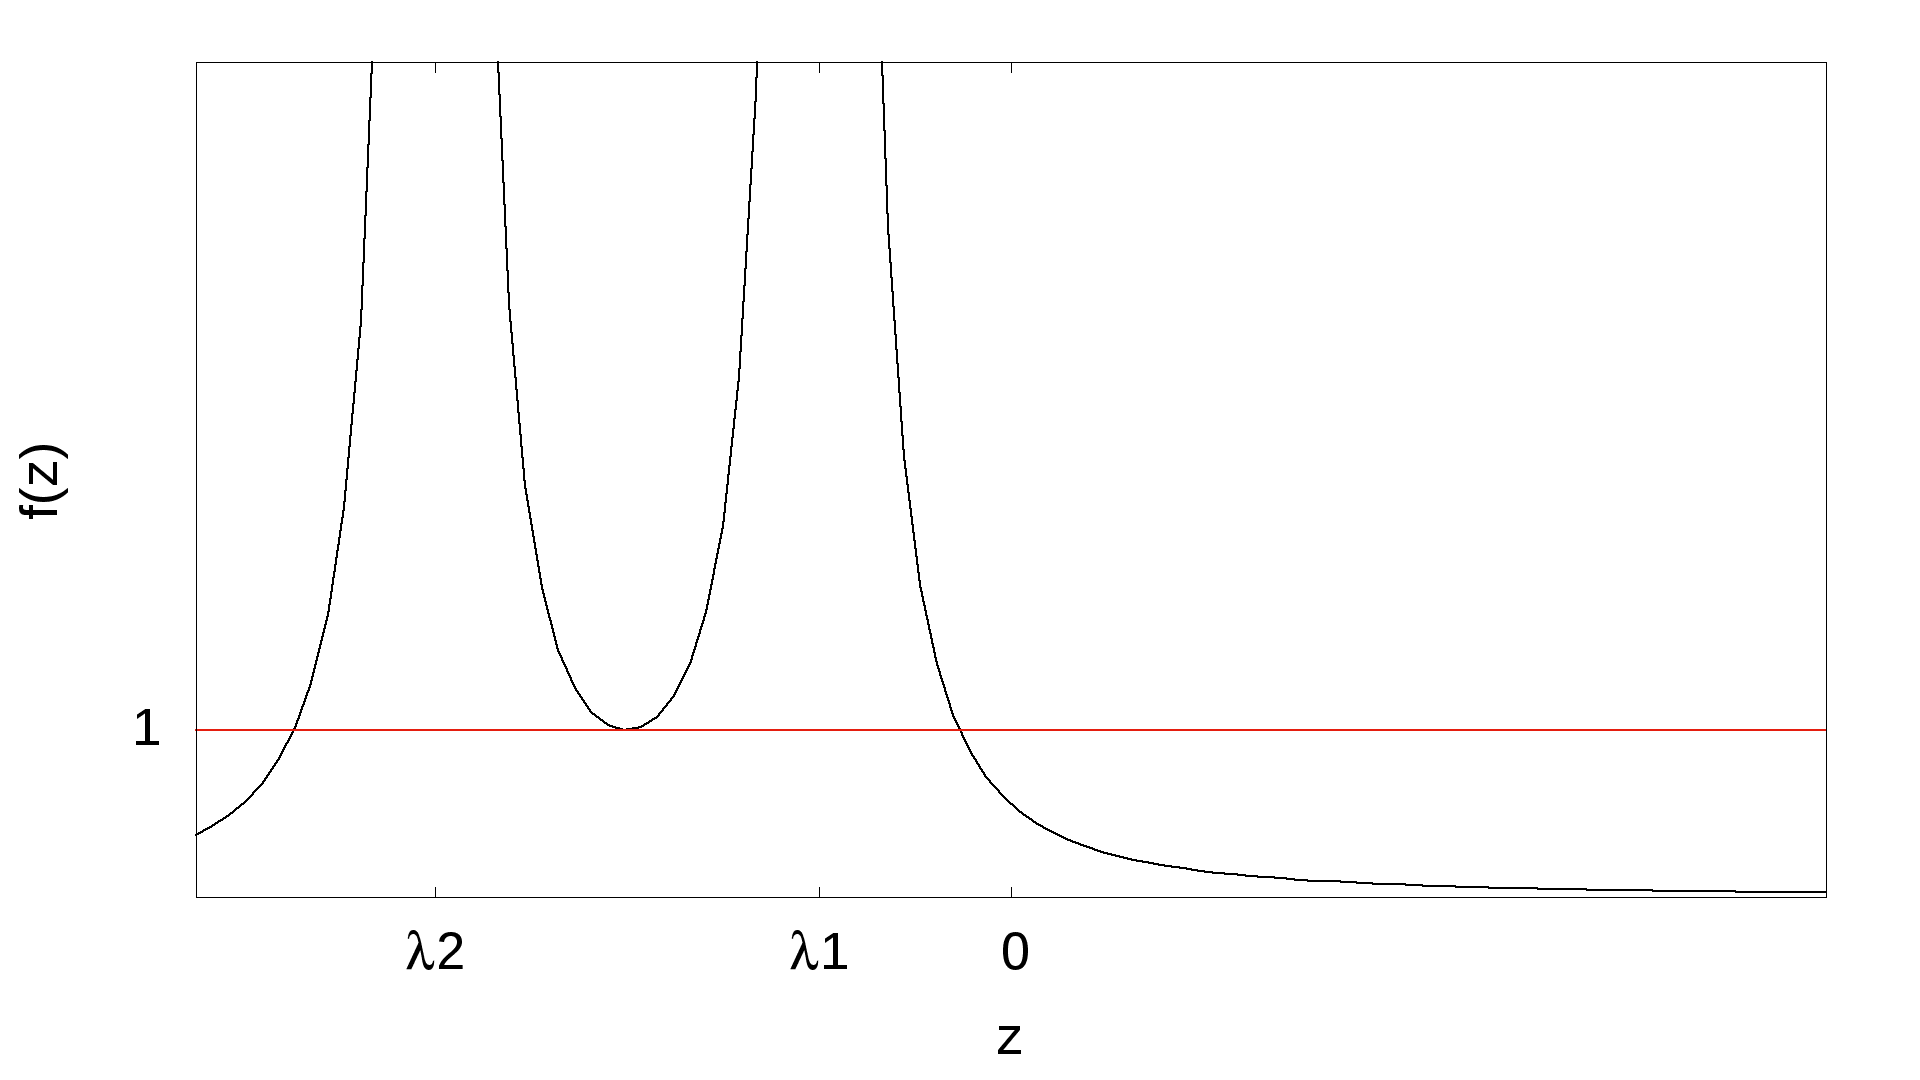
\includegraphics[width=\textwidth]{grafica_lambdas_negativas.png}
 	 \caption{}
 	 \label{fig:lamdas_negativas}
 \end{subfigure}
 
 \begin{subfigure}[b]{0.4\textwidth}
 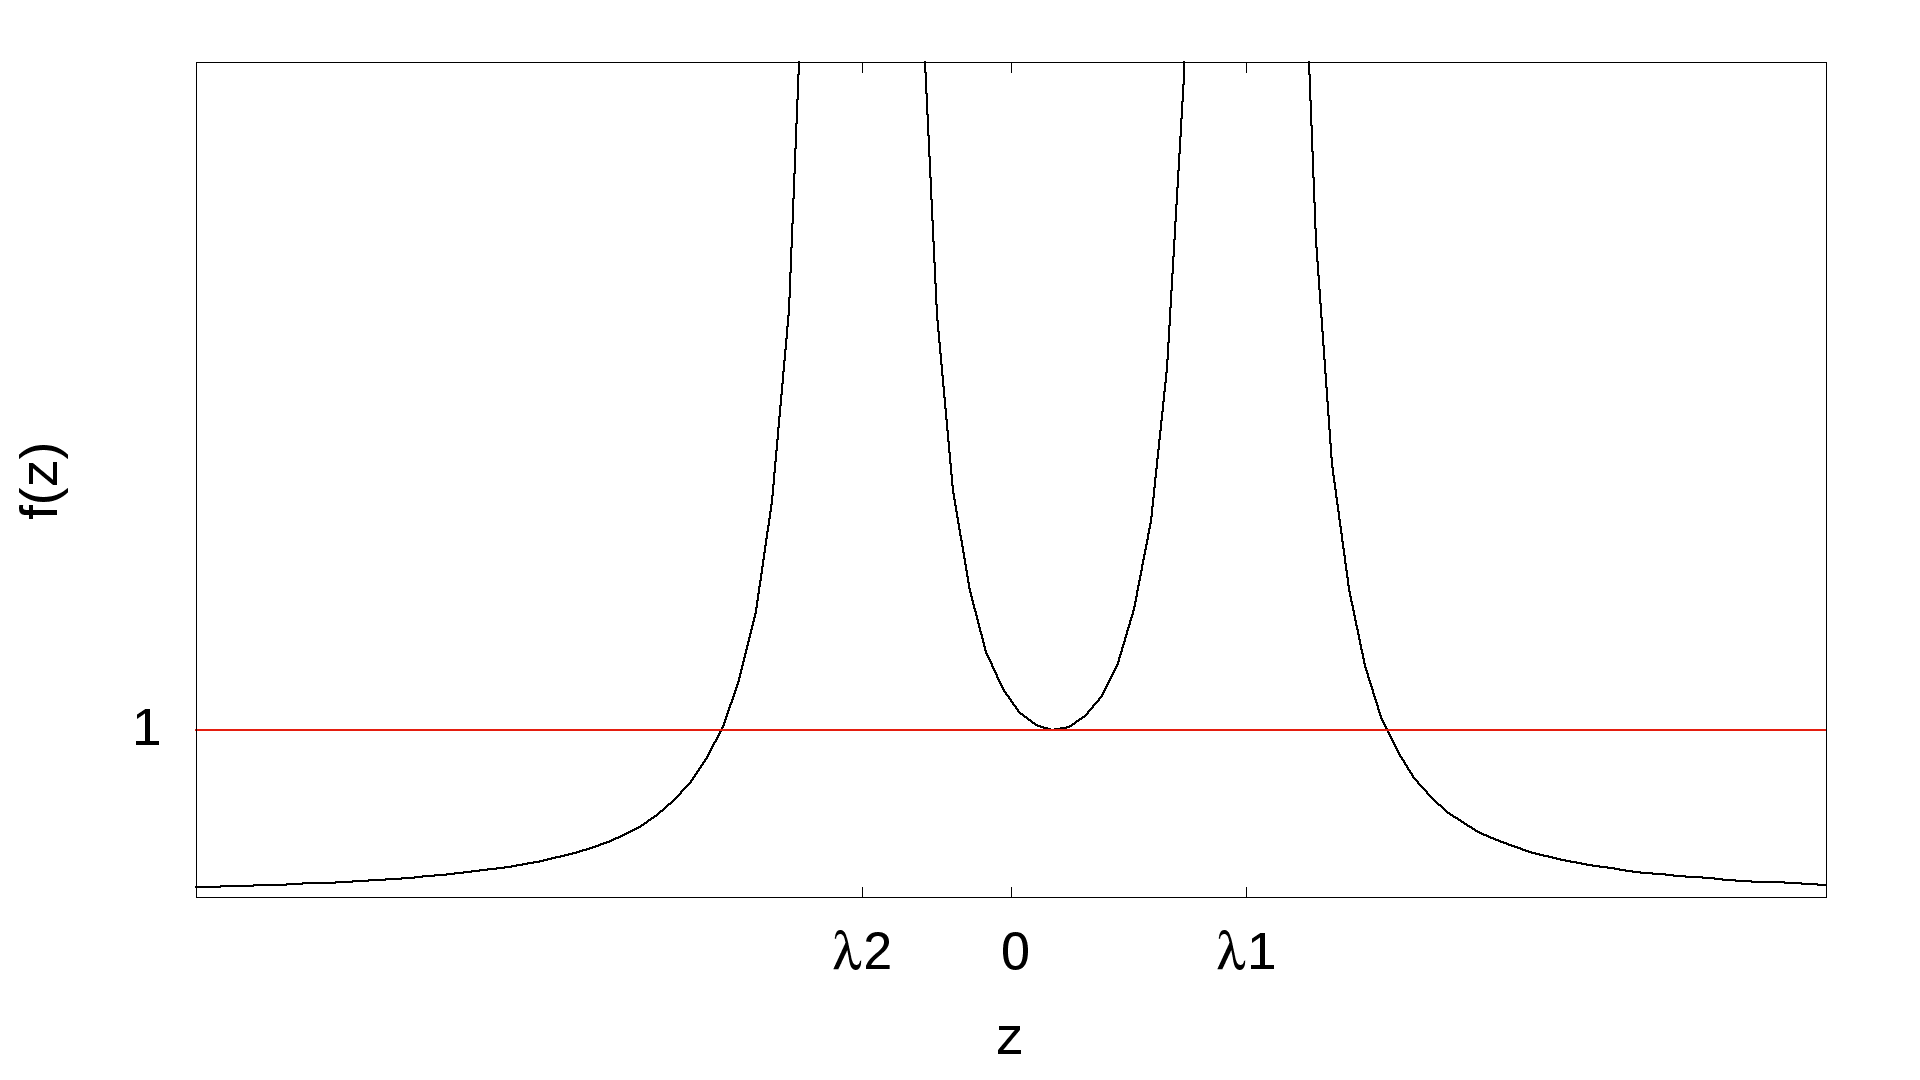
\includegraphics[width=\textwidth]{grafica_lambdas_alternadas.png}
 \caption{}
 \label{fig:lamdas_alternadas}
 \end{subfigure}
 ~
  \begin{subfigure}[b]{0.4\textwidth}
 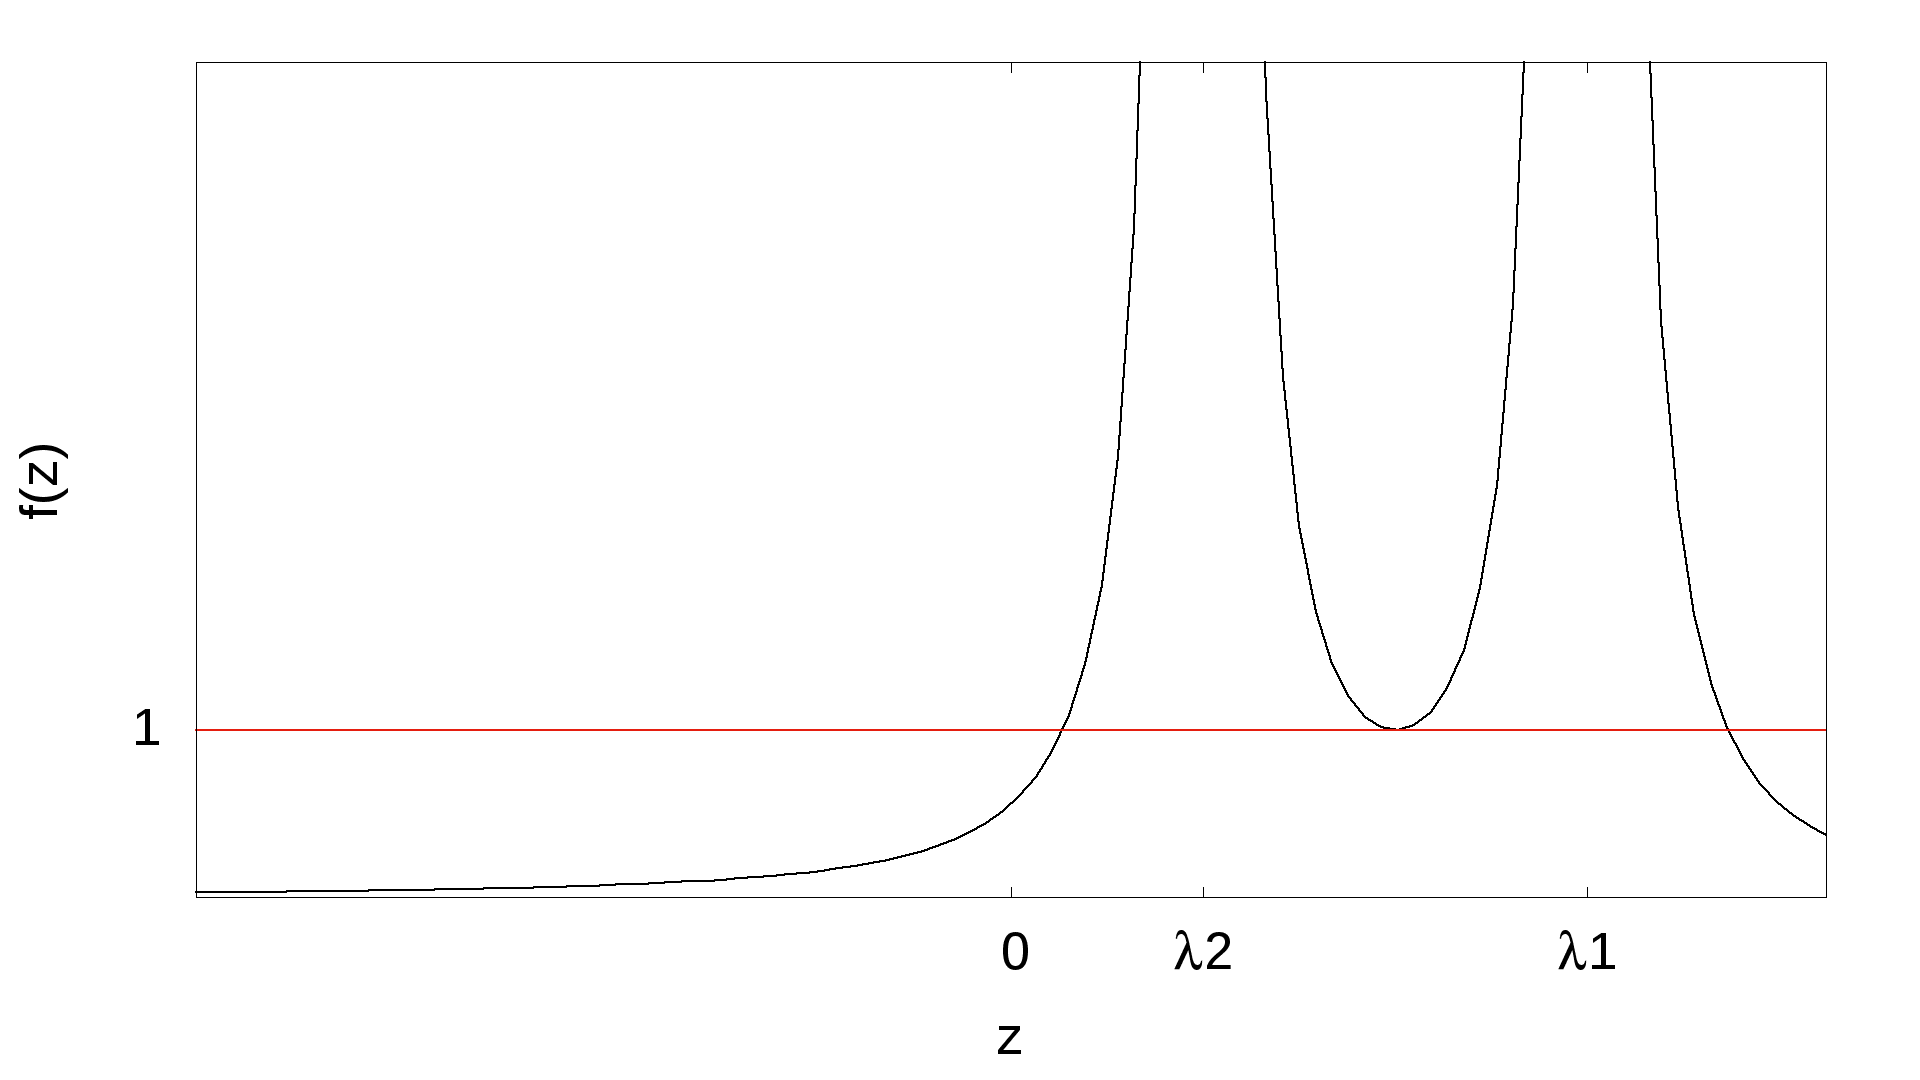
\includegraphics[width=\textwidth]{grafica_lambdas_positivas.png}
  \caption{}
 \label{fig:lamdas_positivas}
 \end{subfigure}
 \caption{Representaciones de los distintos valores que $\lambda_1$ y $\lambda_2$ pueden tomar. Siendo estos cuando ambas son negativas, cuando una es negativa y la otra es positiva y el caso donde ambas son positivas.}\label{fig:valores_lambda}
\end{figure}
Se tiene entonces que se puede definir una distancia $\lambda$ entre $\lambda_1$ y $\lambda_2$ de la forma $\lambda = \lambda_1 - \lambda_2$. La cual permite ver que la ecuación \ref{eq:misma_omega_reposo} es un caso donde $\lambda_2 =0$ y por lo tanto $\lambda_1 = \lambda$. No está de más entonces suponer que si se tiene $\lambda$ constante se puedan recuperar los casos de velocidades opuestas y el de velocidades arbitrarias a partir de una traslación del caso en reposo.\\
Dicha traslación se propone como el cambio de variable $z=z'-\lambda_2$ y recordando que se está tomando $\lambda= \lambda_1 - \lambda_2$ se llega a:
\begin{equation}
\label{eq:misma_omega_general}
1 = \frac{1}{(z'-\lambda_2)^2} + \frac{1}{(z'-\lambda_1)^2}
\end{equation}
Que es el caso general para dos especies con misma $\omega_{p\sigma}$ y velocidades arbitrarias. Lo que la ecuación \ref{eq:misma_omega_general} expone es que el caso de dos velocidades de signo contrario se puede recuperar del caso en reposo ya se haciendo $\lambda_2 = -\lambda_1$ en \ref{eq:misma_omega_general} o realizando el cambio de variable $z=z' +\lambda_1$ y $\lambda= 2\lambda_1$ en \ref{eq:misma_omega_reposo}. Cualquiera de los dos métodos da la expresión:
\begin{equation}
\label{eq:misma_omega_opuestas_cambio}
1 = \frac{1}{(z'+\lambda_1)^2} + \frac{1}{(z'-\lambda_1)^2}
\end{equation}
La cual sabemos se reduce a una ecuación bicuadrática.\\
Del caso de una especie en reposo se tenía que el umbral era:
\begin{equation}
0<\lambda<\sqrt{8}
\end{equation}
Que pasandolo al caso general se tiene:
\begin{equation}
0<\lambda_1 - \lambda_2 <\sqrt{8}
\end{equation}
Por otro lado la máxima tasa de crecmiento sucedía cuando
\begin{equation}
\lambda=\sqrt{3}
\end{equation}
Que resulta ser 
\begin{equation}
\lambda_1 - \lambda_2 = \sqrt{3}
\end{equation}
%\subsection*{Caso con $\omega_{p\sigma}$ diferentes y una especie estacionaria.}
%
\subsection*{Caso D+e - D+e (estacionario e incidente)}
Este caso consiste en núcleos de deuterio y electrones moviendose a una velocidad $\overrightarrow{\textbf{u}}_{\sigma 0}$ incidiendo con un plasma estacionario compuesto de deuterio y electrones. Se trata entonces de un caso de cuatro especies. Cuya relación de dispersión normalizada es de la forma:
\begin{equation}
\label{eq:disp_d-d}
\frac{\epsilon_1}{z^2}+\frac{1}{z^2}+\frac{\epsilon_1}{(z-\lambda)^2}+\frac{1}{(z-\lambda)^2}=1
\end{equation}
Donde $\epsilon_1 = \omega_{pD}/ \omega_{pe}$. Para encontrar el umbral de inestabilidad se realiza el mismo procedimiento de los casos anteriores. Se minimiza la ecuación \ref{eq:disp_d-d} y se resuelve para obtener $z$ en términos de $\lambda$. Que resulta ser $z=\lambda /2$.
\begin{equation}
\frac{\epsilon_1}{z^3}+\frac{1}{z^3}+\frac{\epsilon_1}{(z-\lambda)^3}+\frac{1}{(z-\lambda)^3}=0
\end{equation}
Si se sustituye en \ref{eq:disp_d-d} y se resuelve para $\lambda$ se encuentra entonces que:
\begin{equation}
0 < \lambda < \sqrt{8(1+\epsilon)}
\end{equation}
Para encontrar la máxima tasa de crecimiento se empieza por buscar la raíz del lado derecho de \ref{eq:disp_d-d} que tenga parte imaginaria positiva. Dicha raíz resulta ser:
\begin{equation}
\label{eq:raiz_d-d}
z =\frac{1}{2}\left(\lambda + \sqrt{4 + 4\epsilon + \lambda ^2 -4\sqrt{1+2\epsilon + \epsilon^2+ \lambda^2 + \epsilon \lambda ^2}} \right)
\end{equation}
La cual también se multiplica por su conjugado para así obtener el cuadrado de su componente imaginaria.
\begin{equation}
y^2 = -\left(4 + 4\epsilon + \lambda ^2 -4\sqrt{1+2\epsilon + \epsilon^2+ \lambda^2 + \epsilon \lambda ^2}\right)
\end{equation}
El cual se maximiza con respecto a $\lambda$ y al resolver da $\lambda = \sqrt{3(1 + \epsilon)}$. La cual se sustituye en la ecuación \ref{eq:disp_d-d} para dar:
\begin{equation}
\label{eq:z-max-d-d}
z = \frac{1}{2}\left(\sqrt{3(1+\epsilon)} + i \sqrt{(1+\epsilon)} \right)
\end{equation}
Al tratarse de el caso de deuterio, se tiene que $\epsilon = 2.72 \times 10^{-4}$. Que al sustituir en la ecuación \ref{eq:z-max-d-d} da:
\begin{equation}
z=0.86614 + 0.50007i
\end{equation}
Entonces, el umbral de inestabilidad resulta ser:
\begin{equation}
0 < \lambda < 2.82881
\end{equation}
Y la máxima tasa de crecimiento sucede cuando $\lambda = 1.73229$.
Esto se traduce como:
\begin{equation}
ku_0 < 2.82881 \omega_{pe}
\end{equation}
Para el umbral de inestabilidad.
\begin{equation}
ku_0 = 1.73229 \omega_{pe}
\end{equation}
Para el valor al cual aparece la máxima tasa de crecimiento.
\begin{equation}
\omega = (0.86614 + 0.50007i)\omega_{pe}
\end{equation}
Y finalmente la expresión para la frecuencia cuando ésta ocurre. La figura \ref{fig:d-d} muestra el comportamiento de la parte imaginaria de $z$ para el caso que se acaba de estudiar.
\begin{figure}
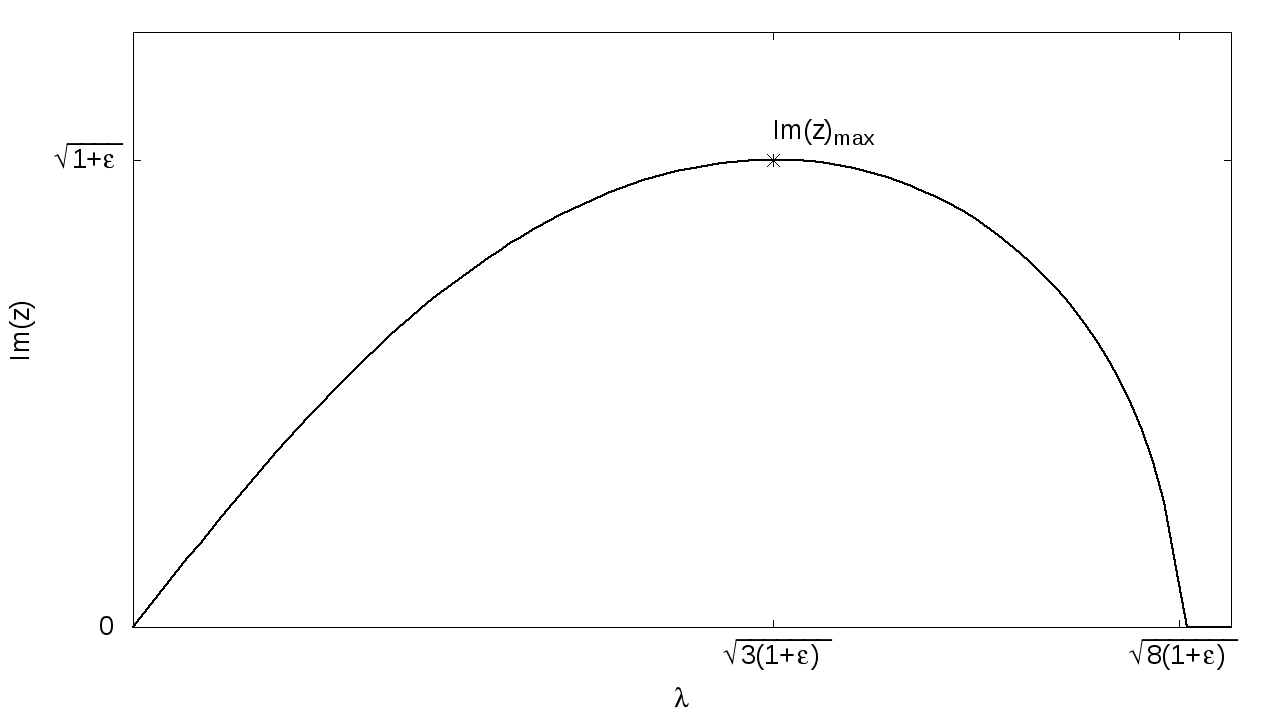
\includegraphics[height=0.3\paperheight]{grafica-d-d-reposo}
\caption{$Im(z)$ en función de $\lambda$, con $\epsilon = 2.72 \times 10^{-4}$ para el caso de un haz de deuterio-electrén incidiendo con un plasma estacionario deuterio-electrón.}
\label{fig:d-d}
\end{figure}
\subsection*{Caso para iones estacionarios y electrones incidentes*}
La relación de dispersión para este caso es la siguiente:
\begin{equation}
\label{eq:disp_ion_electron}
\frac{\epsilon}{z^2}+\frac{1}{(z-\lambda)^2}=1
\end{equation}
Donde $z$ y $\lambda$ son las constantes normalizadas de los casos anteriores, mientras que $\epsilon = m_e/m_i$.
Siguiendo el proceso que se ha estado haciendo, lo primero que se busca es el umbral de inestabilidad. Es decir para que valores de $\lambda$ dos raíces reales colapsan a una sola o aparecen raíces complejas. Como ya se había mencionado, esto sucede cuando el mínimo del lado izquierdo de la ecuación \ref{eq:disp_ion_electron} es mayor o igual a la unidad. Si se toma al lado izqueirdo de \ref{eq:disp_ion_electron} como una función $f(z,\lambda)$ y se minimiza se llega a una expresión:
\begin{equation}
\frac{\epsilon}{z^3}+\frac{1}{(z-\lambda)^3}=0
\end{equation}
De donde se busca tener exponentes positivos para $z$ por lo que se manipula para obtener:
\begin{equation}
\frac{z^3}{\epsilon}=-(z-\lambda)^3
\end{equation}
De donde se pueden obtener raíces cúbicas de cada término:
\begin{equation}
\frac{z}{\epsilon ^{1/3}}=-(z-\lambda)
\end{equation}
De la cual se despeja $z$
\begin{equation}
z_{min}=\frac{\epsilon ^{1/3}\lambda}{(1- \epsilon^{1/3})}
\end{equation}
Que es el valor que la variable $z$ debe tener para que el mínimo sea uno. Está $z_{min}$ se puede substituir en la relación de dispersión para llegar al valor de $\lambda$ que buscamos:
\begin{equation}
1=f(z_{min},\lambda)=\frac{(1+\epsilon^{1/3})^3}{\lambda^2}
\end{equation}
Entonces, para que el mímimo sea mayor o igual a uno el valor de $\lambda$ debe ser:
\begin{equation}
\label{eq:umbral_ion_electron}
\lambda \geq (1+\epsilon^{1/3})^{3/2}
\end{equation}
El cual es nuestro umbral de inestabilidad.
El siguiente paso es entonces buscar una raíz para $z$ en la expresión \ref{eq:disp_ion_electron} que describa el crecimiento de una inestabilidad. Sin embargo, a diferencia de los casos anteriores la ecuación \ref{eq:disp_ion_electron} no se reduce a una ecuación bicuadrática al hacer el cambio de variable y por ello el procedimiento para encontrar la raíz es más laborioso. A continuación se muestra a grandes razgos el cálculo de la raíz, el procedimiento se encuentra con mayor detalle en el apéndice \ref{Ap:raices}.\\
Al expandir la ecuación \ref{eq:disp_ion_electron} y realizando el cambio de vairable $z=x+\frac{\lambda}{2}$ se llega a:
\begin{equation}
x^4 + (-\frac{\lambda^2}{2} -\epsilon -1)x^2 + (\epsilon \lambda - \lambda)x + \frac{\lambda^4}{16}-\frac{\epsilon \lambda^2}{4}-\frac{\lambda^2}{4}=0
\end{equation}
De cuyos coeficientes se construye una expresión para el término auxiliar $\alpha_0$ que es de la forma:
\begin{multline}
\alpha_0 = \frac{1}{3}\left(\frac{\lambda^2}{2} + \epsilon + 1 \right)\\
+ \left(\frac{1}{216}\lbrace-\epsilon^3+3\epsilon^2(\lambda^2-1)-
3\epsilon(\lambda^4 +16\lambda^2 +1)+ (\lambda^2 -1)^3\rbrace \right. \\
\left. +\frac{\lambda}{12\sqrt{3}}\lbrace\epsilon [\epsilon^3-3\epsilon^2(\lambda^2 -1)+3\epsilon(\lambda^4 + 7\lambda^2 +1)- (\lambda^2-1)^3]\rbrace^{1/2} \vphantom{\frac{1}{216}}\right)^{1/3}\\
+ \left(\frac{1}{216}\lbrace-\epsilon^3+3\epsilon^2(\lambda^2-1)-
3\epsilon(\lambda^4 +16\lambda^2 +1)+ (\lambda^2 -1)^3\rbrace \right. \\
\left. -\frac{\lambda}{12\sqrt{3}}\lbrace\epsilon [\epsilon^3-3\epsilon^2(\lambda^2 -1)+3\epsilon(\lambda^4 + 7\lambda^2 +1)- (\lambda^2-1)^3]\rbrace^{1/2} \vphantom{\frac{1}{216}}\right)^{1/3}
\end{multline}
Una vez obtenido $\alpha_0$ se puede encontrar entonces una raíz para $x$ cuya parte imaginaria sea postiva y al volver a realizar un cambio de variable se recupera la raíz para $z$.
\begin{equation}
z= \frac{1}{2} \left( \lambda + \sqrt{2\alpha_0} + \sqrt{2\alpha_0 -4 \left(-\frac{1}{2}(\frac{\lambda^2}{2}+\epsilon+1)+\alpha_0 +\frac{\epsilon \lambda - \lambda}{2\sqrt{2\alpha_0}}\right)}\right)
\end{equation}
\subsection*{Transferencia de energía}
Se empieza con proponer un potencial de onda unidimensional.
\begin{equation}
\label{eq:potencial_sinosoidal}
\Phi(x,t) = \Phi_0 cos(kx-\omega t)
\end{equation}
Esto corresponde a una partícula sobre la cual está actuando una onda que se mueve en la dirección positiva de x con velocidad de fase $\omega /k$. Si se asume que no hay campo magnético, la ecuación de movimento es de la forma:
\begin{equation}
\label{eq:mov_sen_particula}
\frac{dv}{dt}=\frac{qk\Phi_0}{m}sen(kx-\omega t)
\end{equation}
Cuyas condiciones iniciales para un tiempo $t=0$ son $x_0$ y $v_0$. En este caso la $v_0$ se refiere a la velocidad de inyección de la partícula.\\
Se tiene que en el sistema de referencia de la onda, la energía es una constante de movimiento ya que el hamiltoniano es independiente del tiempo en el sistema de referencia de la onda por lo que resultaria conveniente trabajar sobre este. Para ello se introduce la variable $\psi= kx - \omega t$, que viene siendo la fase de la onda en la posición de la partícula. La razón para introducir esta variable es debido a que al hacer $\psi$ la variable dependiente es equivalente a realizar una transformación al sistema de la onda. Por último, resulta más conveniente trabajar con la variable de fase modificada $\theta = kx -\omega t -\pi$, pues evitara lidiar con algunos signos negativos. De esta manera la primera y segunda derivadas de $\theta$ son:
\begin{equation}
\label{eq:deriv_theta}
\frac{d\theta}{dt}=kv -\omega
\end{equation}
\begin{equation}
\label{eq:segunda_deriv_theta}
\frac{d^2\theta}{dt^2}=k \frac{dv}{dt}
\end{equation}
Sustituyendo entonces la ecuación \ref{eq:mov_sen_particula} en la segunda derivada de $\theta$ se obtiene:
\begin{equation}
\label{eq:seg_deriv_theta_sustitucion}
\frac{d^2\theta}{dt^2}=\frac{qk^2\Phi_0}{m}sen(\theta + \pi)
\end{equation}
O bien:
\begin{equation}
\label{eq:seg_deriv_th_simple}
\frac{d^2\theta}{dt^2}+\omega_b sen(\theta)=0
\end{equation}
Donde se ha definido a $\omega_b = qk^2\Phi_0/m$ como la frecuencia de rebote. Si además se define una variable adimensional $\tau = \omega_b t$ como el tiempo normalizado de rebote, la ecuación \ref{eq:seg_deriv_th_simple} se puede escribir como:
\begin{equation}
\label{eq:mov_theta_tau}
\frac{d^2\theta}{d\tau^2}+sen(\theta)=0
\end{equation}
Al estar en el marco de referencia de la onda sería conveniente encontrar una expresión para el hecho de que la energía es una constante de movimiento en el sistema de la onda. Dicha expresión se puede encontrar si se multiplica la ecuación \ref{eq:mov_theta_tau} por el factor integrante $2d\theta/d\tau$.
\begin{equation}
2\frac{d\theta}{d\tau}\frac{d}{d\tau}\left(\frac{d\theta}{d\tau}\right) + 2\frac{d\theta}{d\tau}sen(\theta)=0
\end{equation}
La cual se puede escribir como
\begin{equation}
\label{eq:energia_constante_1}
\frac{d}{d\tau}\left[\left(\frac{d\theta}{d\tau}\right)^2 -2cos(\theta)\right]=0
\end{equation}
Que al integrar da:
\begin{equation}
\label{eq:energia_const_onda}
\left(\frac{d\theta}{d\tau}\right)^2 -2cos(\theta)=\eta=cte
\end{equation}
La ecuación \ref{eq:energia_const_onda} es la expresión para la conservación de la energía que se estaba buscando salvo un factor constante.\\
El término $\eta$ se determina a partir de las condiciones iniciales del sistema las cuales son: la velocidad de inyección en el sistema de referencia de la onda
\begin{equation}
\label{eq:wave_frame_injection_velocity}
\left(\frac{d\theta}{d\tau}\right)_{\tau =0}=\frac{1}{\omega_b}\left(\frac{d\theta}{dt}\right)_{t=0}=\frac{1}{\omega_b}(kv_0-\omega)=\alpha
\end{equation}
Y la fase de inyección en el sistema de referencia de la onda
\begin{equation}
\label{eq:wave_frame_injection_phase}
\theta_{\tau=0}=kx_0-\pi=\theta_0
\end{equation}
Por lo que $\eta$ se puede expresar como
\begin{equation}
\label{eq:expresion_eta_wave_frame}
\eta = \alpha^2 -2cos(\theta_0)
\end{equation}
Como ya se habia mencionado, $\eta$,$\alpha^2$ y $-2cos(\theta_0)$ son términos para la energía total, cinética y potencial respectivamente salvo un factor constante en el sistema de la onda.\\
Al ser términos referentes a la energía, $\alpha^2$ y $-2cos(\theta_0)$, o mejor dicho la relación entre esos términos, dan información acerca del comportamiento de la partícula sujeta al potencial que se definió al principio. En particular se hablará se cuando una partícula está atrapada en alguna región del potencial, lo cual corresponderá al caso cuando la energía cinética de la partícula es menor que la energía potencial, y el caso en el que la partícula no se encuentra atrapada por el potencial, es decir que su energía cinética es mayor que la energía potencial.\\
De la ecuación \ref{eq:expresion_eta_wave_frame} se tiene entonces
\begin{itemize}
\item Si $\alpha^2 < |2cos(\theta_0)| \Rightarrow -2<\eta<2$ y se habla de una partícula atrapada.
\item Si $\alpha^2 > |2cos(\theta_0)| \Rightarrow \eta>2$ y se habla de una partícula no atrapada y que se me mueve continuamente en una dirección pero cuya velocidad se verá afectada dependiendo de en que parte del potencial se encuentre.
\end{itemize}
Por el momento se considera solamente el caso donde la energía cinética de la partícula es mucho mayor que la energía potencial, es decir cuando $\alpha^2 \gg 2$ y se buscará determinar la manera en la que estas partículas no atrapadas intercambian energía con la onda. Cabe mencionar, que dadas las definiciones de $\alpha$, ecuación \ref{eq:wave_frame_injection_velocity}, y de $\omega_b$, se tiene $\alpha^2 \sim \Phi_0^{-1}$ por lo que un valor de $\alpha^2 \gg 2$ implica un valor para $\Phi_0 \ll 2$. Donde $\Phi_0$ viene siendo la amplitud de la onda. Por lo que el caso que se va a estudiar corresponde a ondas con amplitudes pequeñas.\\
Para poder determinar la energía transferida entre la onda y la partícula se debe poder expresar la energía cinética de la partícula en términos de cantidades del sistema de la onda. Para ello se utiliza la ecuación \ref{eq:deriv_theta} y la definición de $\tau$ para primero despejar la velocidad en el sistema del laboratorio y luego expresarla en términos de cantidades encontradas en el sistema de la onda.
\begin{equation}
\label{eq:velocidad_lab_transferencia}
v =\frac{1}{k}\left(\omega +\frac{d\theta}{dt}\right)= \frac{\omega_b}{k}\left(\frac{\omega}{\omega_b} +\frac{d\theta}{d\tau}\right)
\end{equation}
Entonces, la energía cinética se puede expresar como
\begin{equation}
\label{eq:energia_cintetica_1}
W = \frac{1}{2}mv^2=\frac{m\omega_b^2}{2k^2}\left[\frac{\omega^2}{\omega_b^2}+2\frac{\omega}{\omega_b}\frac{d\theta}{d\tau}+\left(\frac{d\theta}{d\tau}\right)^2\right]
\end{equation}
El término cuadrático de la derivada se puede sustitur utilizando la ecuación \ref{eq:energia_const_onda} y entonces la energía cinética de la partícula está dada por:
\begin{equation}
\label{eq:energia_cinetica_2}
W = \frac{m\omega_b^2}{2k^2}\left[\frac{\omega^2}{\omega_b^2}+2\frac{\omega}{\omega_b}\frac{d\theta}{d\tau}+\eta+ 2cos(\theta)\right]
\end{equation}
El siguiente paso es entonces determinar como va variando $W$ con respecto del tiempo
\begin{equation}
\label{eq:derivada_temp_W_1}
\frac{dW}{dt}=\frac{m\omega_b^3}{k^2}\left[\frac{\omega}{\omega_b}\frac{d^2\theta}{d\tau^2}-2\frac{d\theta}{d\tau}sen(\theta)\right]=-\frac{m\omega_b^3}{k^2}sen(\theta)\left[\frac{\omega}{\omega_b}+\frac{d\theta}{d\tau}\right]
\end{equation}
Donde se ha vuelto a utlizar la definición de $\tau$, junto con la regla de la cadena y la ecuación \ref{eq:mov_theta_tau}.\\
Lo que prosigue es encontrar la dependencia temporal de 
%y el proceso se complica. Para solventar este problema se hara uso de una expansión de Taylor alrededor de $(z_{min},\lambda)$ es decir:
%\begin{equation}
%\label{eq:expansion_ion_electron}
%f(z,\lambda)=f(z_{min},\lambda) + f_z(z_{min},\lambda)(z-z_{min}) + f_{\lambda}(z_{min},\lambda)(\lambda-\lambda)+ \frac{1}{2}f_{zz}(z_{min},\lambda)(z-z_{min})^2
%\end{equation}
%Donde $f_z(z_{min},\lambda)=0$ y la derivada con respecto a $\lambda$ se cancela porque está siendo multiplicada por un cero. La ecuación \ref{eq:expansion_ion_electron} se reduce a:
%\begin{equation}
%\label{eq:reduc_ion_electron}
%1=f(z,\lambda)=f(z_{min},\lambda)+ \frac{1}{2}f_{zz}(z_{min},\lambda)(z-z_{min})^2
%\end{equation}
%El siguiente paso es entonces despejar $z$. Simple manipulación algebraica nos lleva a:
%\begin{equation}
%(z-z_{min})^2 =\frac{2(1-f(z_{min},\lambda))}{f_{zz}(z_{min},\lambda)}
%\end{equation}
%Ahora bien, si se asume $f(z_{min},\lambda)) > 1$ entonces al sacar raíz cuadrada se tiene:
%\begin{equation}
%z=z_{min} \pm \sqrt{2}i\left(\frac{f(z_{min},\lambda)-1}{f_{zz}(z_{min},\lambda)} \right)^{1/2}
%\end{equation}
%Donde:
%\begin{equation}
%f_{zz}(z_{min},\lambda)=\frac{-3(\epsilon^{1/3} -1)^4}{\lambda^4}\left(\frac{\epsilon^{1/3}+(1-2\epsilon^{1/3})^4}{\epsilon^{1/3}(1-2\epsilon^{1/3})^4}\right)
%\end{equation}
%Sustituyendo entonces se obtiene:
%\begin{equation}
%z=\frac{\epsilon ^{1/3}\lambda}{(1- \epsilon^{1/3})} + \frac{i}{\sqrt{3}}\left(\frac{\lambda \epsilon^{1/6}(2\epsilon^{1/3}-1)^2((1-\epsilon^{1/3})^3-\lambda^2)^{1/2}}{(\epsilon^{1/3}-1)^2(\epsilon^{1/3}+(2\epsilon^{1/3}-1)^4)^{1/2}}\right)
%\end{equation}
\appendix
\numberwithin{equation}{section}
\section{Cálculo de raices}\label{Ap:raices}
\subsection*{Resolviendo ecuaciones cuárticas.}
Un método para resolver ecuaciones cuárticas es el llamado método de Ferrari \cite{higheralgebra} y prosigue de la siguiente manera. Si se parte de la forma general de la ecuación cuártica, es decir:
\begin{equation}
z^4 +az^3+bz^2+cz+d=0
\label{eq:general_cuartica}
\end{equation}
Entonces, se propone el cambio de variable $z=x-\frac{a}{4}$, lo que da como resultado:
\begin{multline}
x^4-ax^3+\frac{3}{8}a^2x^2-\frac{1}{16}a^3x+\frac{1}{256}a^4 +ax^3 - \frac{3}{4}a^2x^2 + \frac{3}{16}a^3x \\
-\frac{1}{64}a^4 + bx^2 -\frac{1}{2}abx+ \frac{1}{16}a^2b + cx -\frac{1}{4}ac +d =0
\end{multline}
Que al agrupar términos queda:
\begin{equation}
x^4+\left(b-\frac{3}{8}a^2\right)x^2 + \left(\frac{1}{8}a^3-\frac{1}{2}ab +c\right)x+ \left(d-\frac{1}{4}ac +\frac{1}{16}a^2b-\frac{3}{256}a^4\right)
\end{equation}
Se llega entonces a una ecuación cuártica reducida, de la forma:
\begin{equation}
x^4 +px^2+qx+r=0
\label{eq:cuartica_reducida}
\end{equation}
El siguiente paso en introducir un término auxiliar $\alpha$, por lo que se reescribe la ecuación \ref{eq:cuartica_reducida} como:
\begin{equation}
x^4 +px^2+qx+r=\left(x^2 +\frac{p}{2}+\alpha\right)^2 +qx+r -\frac{p^2}{4}-\alpha^2 -2x^2\alpha -p\alpha=0
\end{equation}
O bien:
\begin{equation}
\label{eq:cuartica_alpha}
\left(x^2 +\frac{p}{2}+\alpha\right)^2 - \left[2\alpha x^2 -qx + \left(\alpha^2 +p\alpha-r +\frac{p^2}{4}\right)\right]=0
\end{equation}
Entonces, se escoge el valor de $\alpha$ tal que complete el cuadrado dentro de los corchetes. Esto es que tenga una raíz doble, por lo que su discriminante sería cero. Se requiere entonces que $\alpha$ cumpla con:
\begin{equation}
\label{eq:discriminante_cuartica_reducida}
q^2 -4 \cdot 2\alpha \left(\alpha^2 +p\alpha-r +\frac{p^2}{4}\right)=0
\end{equation}
La cual es una ecuación cúbica con tres raíces. Tomamos entonces una de esas raíces, por ejemplo $\alpha_0$. Se tiene entonces que la raíz dentro de los corchetes es $q/4\alpha_0$. Por lo que la ecuación \ref{eq:cuartica_alpha} se reescribe como:
\begin{equation}
\left(x^2 +\frac{p}{2}+\alpha\right)^2 -2\alpha_0 \left(x -\frac{q}{4\alpha_0}\right)^2=0
\end{equation}
La cual es una diferencia de cuadrados. Entonces podemos ver ecuación anterior como:
\begin{equation}
\left(x^2 + \frac{p}{2}+\alpha_0 - \sqrt{2}\alpha_0 \left(x-\frac{q}{4\alpha_0}\right)\right)\left(x^2 + \frac{p}{2}+\alpha_0 + \sqrt{2}\alpha_0 \left(x-\frac{q}{4\alpha_0}\right)\right)=0
\end{equation}
Se llega entonces a dos raíces cuadráticas:
\begin{equation}
\label{eq:cuartica_cuadratica1}
x^2 -\sqrt{2\alpha_0}x+\left(\frac{p}{2}+\alpha_0 + \frac{q}{2\sqrt{2\alpha_0}}\right)=0
\end{equation}
\begin{equation}
\label{eq:cuartica_cuadratica2}
x^2 +\sqrt{2\alpha_0}x+\left(\frac{p}{2}+\alpha_0 - \frac{q}{2\sqrt{2\alpha_0}}\right)=0
\end{equation}
De las cuales se pueden encontrar sus dos raíces, que debido a que se llegó a \ref{eq:cuartica_cuadratica1} y a \ref{eq:cuartica_cuadratica2} por medio de identidades, resultan ser raíces de la ecuación \ref{eq:cuartica_reducida}, de la cual se pueden recuperar las raíces de \ref{eq:general_cuartica} al aplicar el cambio de variable.\\
La forma explícita de las raíces de \ref{eq:cuartica_cuadratica1} y \ref{eq:cuartica_cuadratica2} son:
\begin{equation}
x = \frac{1}{2}\left(\sqrt{2\alpha_0} \pm \sqrt{2\alpha_0 - 4\left(\frac{p}{2} + \alpha_0 + \frac{q}{2\sqrt{2\alpha_0}}\right)}\right)
\end{equation}
\begin{equation}
x = \frac{1}{2}\left(-\sqrt{2\alpha_0} \pm \sqrt{2\alpha_0 - 4\left(\frac{p}{2} + \alpha_0 - \frac{q}{2\sqrt{2\alpha_0}}\right)}\right)
\end{equation}
Que al aplicar el cambio de variable resulta en:
\begin{equation}
\label{eq:raiz_12_cuartica}
z_{1,2}= \frac{1}{2} \left(-\frac{a}{2} + \sqrt{2\alpha_0} \pm \sqrt{2\alpha_0 - 4\left(\frac{p}{2} + \alpha_0 + \frac{q}{2\sqrt{2\alpha_0}}\right)}\right)
\end{equation}
\begin{equation}
\label{eq;raiz_34_cuartica}
z_{3,4}= \frac{1}{2} \left(-\frac{a}{2} - \sqrt{2\alpha_0} \pm \sqrt{2\alpha_0 - 4\left(\frac{p}{2} + \alpha_0 - \frac{q}{2\sqrt{2\alpha_0}}\right)}\right)
\end{equation}
Donde se recuerda que 
\begin{align}
\label{eq:valores_p_cuartica}
p&=\left(b-\frac{3}{8}a^2\right)\\
\label{eq:valores_q_cuartica}
q&=\left(\frac{1}{8}a^3 - \frac{1}{2}ab + c \right)
\end{align}
La expresión explícita de $\alpha_0$ se obtiene a partir de la llamada ecuación de Cardan \cite{higheralgebra}. El procedimiento es el siguiente:\\
Partiendo de la ecuación \ref{eq:discriminante_cuartica_reducida}, la cual es una ecuación cúbica.
\begin{equation}
\alpha_0^3 + p\alpha_0^2+ \alpha_0 \left(\frac{p^2}{4}-r\right) - \frac{q^2}{8}=0
\end{equation}
Se vuelve a usar un cambio de variable similar al de la ecuación cuártica de la forma $\alpha_0 = y- \frac{p}{3}$.
\begin{equation}
\label{eq:cubica_camb_var}
y^3 +y\left(-\frac{p^2}{12}-r\right) + \left(\frac{pr}{3}-\frac{q^2}{8}-\frac{p^3}{108}\right)=0
\end{equation}
Ahora bien, si nombramos
\begin{align}
\label{eq:pp_alpha}
p'&=\left(-\frac{p^2}{12}-r\right)\\
\label{eq:qp_alpha}
q'&=\left(\frac{pr}{3}-\frac{q^2}{8}-\frac{p^3}{108}\right)
\end{align}
La ecuación \ref{eq:cubica_camb_var} se puede reescribir entonces como:
\begin{equation}
\label{eq:cub_red}
y^3 +p'y+q'=0
\end{equation}
Donde la ecuación de Cardan \cite{higheralgebra} índica que las raíces son de la forma:
\begin{equation}
y = \left(-\frac{q'}{2} + \sqrt{\frac{q^{'2}}{4}+\frac{p^{'3}}{27}}\right)^{1/3} + \left(-\frac{q'}{2} - \sqrt{\frac{q^{'2}}{4}+\frac{p^{'3}}{27}}\right)^{1/3}
\end{equation}
Entonces, al recuperar el cambio de variable se tiene:
\begin{equation}
\label{eq:alpha_cero}
\alpha_0 = \left(-\frac{q'}{2} + \sqrt{\frac{q^{'2}}{4}+\frac{p^{'3}}{27}}\right)^{1/3} + \left(-\frac{q'}{2} - \sqrt{\frac{q^{'2}}{4}+\frac{p^{'3}}{27}}\right)^{1/3} - \frac{p}{3}
\end{equation}
Se recuerda también que:
\begin{equation}
r= \left(d-\frac{1}{4}ac +\frac{1}{16}a^2b-\frac{3}{256}a^4\right)
\end{equation}
Por último, cabe mencionar que $\alpha_0$ se obtiene de la suma de dos raíces cúbicas, es decir de la forma:
\begin{equation}
\alpha_0 = s +t - \frac{p}{3}
\end{equation}
Se tiene entonces que para obtener un valor válido de $\alpha_0$ solo se pueden escoger ciertos valores de los tres posibles para $s$ y $t$. Estos valores son:
\begin{align}
\label{eq:raices_permitidas_para_aplha}
\alpha_0&=s_1+t_1- \frac{p}{3}\\
\alpha_0&=s_2+t_3- \frac{p}{3}\\
\alpha_0&=s_3+t_2- \frac{p}{3}
\end{align}
\subsection*{Caso misma $\omega_{p\sigma}$ con una especie incidente y la otra estacionaria.}
Expandiendo la ecuación \ref{eq:misma_omega_reposo} se obtiene:
\begin{equation}
\label{eq:misma_omega_expand}
z^4 -2\lambda z^3 +(\lambda^2 -2)z^2 + 2\lambda z -\lambda^2=0
\end{equation}
Para resolver está ecuación se sigue entonces el método de Ferrari, donde se empieza por el cambio de variable $z=x+\frac{\lambda}{2}$, para obtener una expresión simplificada
\begin{equation}
x^4 - \frac{1}{2}(4 + \lambda^2)x^2 + \frac{1}{16}\lambda^2 (\lambda^2 -8)=0
\end{equation}
Donde, al recordar la ecuación \ref{eq:valores_q_cuartica} se tiene que el término de primer orden se cancela. Pues $q=-\lambda^3 + \lambda (\lambda^2 -2) +\lambda$. De esto, se obtiene lo que resulta ser una ecuación bicuadrática, es decir una expresión cuadrática para $x^2$. Cuyas raíces son entonces:
\begin{equation}
x^2 = \frac{1}{4}(4 + \lambda^2 \pm 4\sqrt{ \lambda^2 +1})
\end{equation}
Por lo que las raíces cuárticas son:
\begin{equation}
x= \pm \frac{1}{2}\sqrt{4 + \lambda^2 \pm 4\sqrt{ \lambda^2 +1}}
\end{equation}
Que recordando el cambio de variable se recupera entonces las raíces para la ecuación \ref{eq:misma_omega_expand}.
\begin{equation}
z = \frac{1}{2}\left(\lambda \pm \sqrt{4 + \lambda^2 \pm 4\sqrt{ \lambda^2 +1}}\right)
\end{equation}
Ahora bien, la elección de signos es de acuerdo a la necesidad de una solución con su parte imaginaria positiva, la cual se obtiene tomando el primer signo como positivo y el segundo como negativo.
\subsection*{Caso D+e - D+e (estacionario e incidente)}
Al expandir la ecuación \ref{eq:disp_d-d} se obtiene:
\begin{equation}
z^4 -2\lambda z^3+ (\lambda^2 -2 - 2\epsilon_1)z^2 + (2\lambda+\epsilon_1 \lambda)z+ \lambda^2 (-1 -\epsilon_1)=0
\end{equation}
Y nuevamente haciendo la sustitución $z=x + \frac{ \lambda}{2}$ se obtiene:
\begin{multline}
x^4+2x^3\lambda + \frac{3}{2}x^2 \lambda^2 + \frac{1}{2}x\lambda^3 +\frac{1}{16}\lambda^4 -2x^3 \lambda -3x^2 \lambda^2 - \frac{3}{2}x\lambda^3 - \frac{1}{4}\lambda^4 +x^2\lambda^2 + x\lambda^3 +\frac{1}{4}\lambda^4\\ 
  -2x^2-2x\lambda -\frac{1}{2}\lambda^2 - 2x^2 \epsilon_1-2x\lambda\epsilon_1-\frac{1}{2}\lambda^2\epsilon_1+2x\lambda+2x\epsilon_1\lambda + \lambda^2 \epsilon_1\lambda^2+\lambda^2(-1-\epsilon_1)=0
\end{multline}
La cual se puede reescribir como:
\begin{equation}
x^4 -\frac{1}{2}(\lambda^2 +4\epsilon_1 + 4)x^2 + \frac{1}{16}\lambda^2(\lambda^2 - 8\epsilon -8)=0
\end{equation}
La cual resulta una ecuación bicuártica, se puede entonces sacar para $x^2$ el siguiente resultado:
\begin{equation}
x^2 = \frac{1}{4}\left(4+4\epsilon_1+\lambda^2 \pm 4\sqrt{1+2\epsilon_1+\epsilon_1^2 + \lambda^2+\epsilon_1\lambda^2}\right)
\end{equation}
Se tiene entonces que $x$ es:
\begin{equation}
x=\pm \frac{1}{2} \sqrt{4+4\epsilon_1+\lambda^2 \pm 4\sqrt{1+2\epsilon_1+\epsilon_1^2 + \lambda^2+\epsilon_1\lambda^2}}
\end{equation}
Y recuperando la variable $z$ se tiene que las raíces son de la forma:
\begin{equation}
z = \frac{1}{2}\left(\lambda \pm \sqrt{4+4\epsilon_1+\lambda^2 \pm 4\sqrt{1+2\epsilon_1+\epsilon_1^2 + \lambda^2+\epsilon_1\lambda^2}}\right)
\end{equation}
\subsection*{Caso con especies de $\omega_{p\sigma}$ diferentes con una incidente y la otra en reposo.}
La ecuación a resolver es de la forma:
\begin{equation}
\label{eq:dif_omega_reposo_incidente_cuartica}
z^4 - 2\lambda z^3 + z^2(\lambda^2 -\epsilon -1) +2\epsilon \lambda z - \lambda^2
\epsilon =0
\end{equation}
Entonces, al aplicar el cambio de variable $z=x+\frac{\lambda}{2}$ queda:
\begin{equation}
x^4 + (-\frac{\lambda^2}{2} -\epsilon -1)x^2 + (\epsilon \lambda - \lambda)x + \frac{\lambda^4}{16}-\frac{\epsilon \lambda^2}{4}-\frac{\lambda^2}{4}=0
\end{equation}
Donde los coeficientes $p$,$q$ y $r$ son entonces:
\begin{align}
p&=-\frac{\lambda^2}{2} -\epsilon -1\\
q&=\epsilon \lambda - \lambda\\
r&=\frac{\lambda^4}{16}-\frac{\epsilon \lambda^2}{4}-\frac{\lambda^2}{4}
\end{align}
A diferencia de los casos anteriores, la ecuación \ref{eq:dif_omega_reposo_incidente_cuartica} no se reduce a una bicuadrática por lo que se tiene que las raíces de $z$ están expresadas ya sea por la ecuación \ref{eq:raiz_12_cuartica} o por la ecuación \ref{eq;raiz_34_cuartica} que se encuentran expresadas en términos de los coeficientes $p$,$q$ y un término $\alpha_0$.\\
El siguiente paso es entonces encontrar una expresión explícita para $\alpha_0$ la cual debe ser de la misma forma que la ecuación \ref{eq:alpha_cero} que a su vez está expresada en términos de los coeficientes $p'$ y $q'$ los cuales están definidos por las ecuaciones \ref{eq:pp_alpha} y \ref{eq:qp_alpha}. Para este caso se tiene entonces que $p'$ y $q'$ son:
\begin{align}
\label{eq:pp_alpha_diferente_omega_reposo}
p'&= -\frac{1}{12}\left(1+\epsilon-\lambda^2\right)^2\\
\label{eq:qp_alpha_diferente_omega_reposo}
q'&= \frac{1}{108} \left[ \epsilon^3 -3\epsilon^2 (\lambda^2
-1)+3\epsilon(\lambda^4 + 16\lambda^2 +1)- (\lambda^2 -1)^3 \right]
\end{align}
$\alpha_0$ es entonces:
\begin{multline}
\label{eq:alpha_diferentes_omegas_reposo}
\alpha_0 = \frac{1}{3}\left(\frac{\lambda^2}{2} + \epsilon + 1 \right)\\
+ \left(\frac{1}{216}\lbrace-\epsilon^3+3\epsilon^2(\lambda^2-1)-
3\epsilon(\lambda^4 +16\lambda^2 +1)+ (\lambda^2 -1)^3\rbrace \right. \\
\left. +\frac{\lambda}{12\sqrt{3}}\lbrace\epsilon [\epsilon^3-3\epsilon^2(\lambda^2 -1)+3\epsilon(\lambda^4 + 7\lambda^2 +1)- (\lambda^2-1)^3]\rbrace^{1/2} \vphantom{\frac{1}{216}}\right)^{1/3}\\
+ \left(\frac{1}{216}\lbrace-\epsilon^3+3\epsilon^2(\lambda^2-1)-
3\epsilon(\lambda^4 +16\lambda^2 +1)+ (\lambda^2 -1)^3\rbrace \right. \\
\left. -\frac{\lambda}{12\sqrt{3}}\lbrace\epsilon [\epsilon^3-3\epsilon^2(\lambda^2 -1)+3\epsilon(\lambda^4 + 7\lambda^2 +1)- (\lambda^2-1)^3]\rbrace^{1/2} \vphantom{\frac{1}{216}}\right)^{1/3}
\end{multline}
En caso de que los términos elevados a la $1/3$ sean complejos, nótese que son el conjugado del otro, de esta manera, la expresión \ref{eq:raices_permitidas_para_aplha} nos permite seleccionar las raíces de estos términos de tal manera que se cancele su parte imaginaria haciendo así a $\alpha_0$ un número real.\\
Recordando entonces que la raíz de interes es aquella cuya parte imaginaria sea positiva, se escogen los signos postivos en la ecuación \ref{eq:raiz_12_cuartica} y se sutituyen los coeficientes $p$ y $q$. Queda entonces que la raíz es:
\begin{equation}
\label{eq:raiz_diferente_omega_reposo}
z= \frac{1}{2} \left( \lambda + \sqrt{2\alpha_0} + \sqrt{2\alpha_0 -4 \left(-\frac{1}{2}(\frac{\lambda^2}{2}+\epsilon+1)+\alpha_0 +\frac{\epsilon \lambda - \lambda}{2\sqrt{2\alpha_0}}\right)}\right)
\end{equation}
Donde $\alpha_0$ no se sustituye por simplicidad.
\bibliographystyle{unsrt} 
\bibliography{referencias}

\end{document}
